\documentclass[]{article}
\usepackage[utf8]{inputenc}
\usepackage[T1]{fontenc}
\usepackage{graphicx}
\usepackage[portuguese]{babel}

%opening
\title{Projeto POO - Implementação do Pac-Man}
\author{11011716 - André Aranovich Florentino\\ 11003216 - Bruno Tatsuya Masunaga Santos\\ 11076916 - Lucas Eduardo Gonçalves da Rosa\\ 11006216 - Wesley Pereira da Silva}
\date{\today}

\begin{document}

\maketitle

\centerline{\textbf{Turma: A2 - Matutino}}

\section{Introdução}

Neste trabalho, foi realizado o desenvolvimento de um jogo baseado no clássico dos arcades: Pac-Man. Para tanto, utilizou-se o terminal do Linux como a janela onde o jogo é exibido. O trabalho foi realizado com a intenção de se utilizar conceitos abordados nas aulas da disciplina Programação Orientada a Objetos, ministrada pelos professores Paulo H. Pisani e Saul C. Leite.

O objetivo principal no desenvolvimento do projeto foi criar uma versão do Pac-Man onde arquivos de mapa (em formato .txt) são lidos pelo programa para gerar uma matriz. Neste matriz, ocorre toda a dinâmica do jogo, que pode receber parâmetros como a quantidade de fantasmas contidas no mapa, o mapa a ser jogado e a dificuldade. Tais parâmetros tornam o jogo uma experiência customizável, atendendo, desta forma, as exigências iniciais do trabalho.

\section{Descrição das classes}
Neste projeto, as classes foram criadas com a intenção de implementar a seguinte ideia de modelagem: 

\begin{itemize}
	\item \textbf{GameManager}: É a classe que controla todo o fluxo do jogo. Possui métodos responsáveis pela impressão de movimentação dos elementos ao longo do mapa e de controle de vidas e pontos, além de instanciar todas as demais classes (exceto Principal, Simbolo e Paleta). De modo geral, é a classe que controla funcionalmente o jogo. 
	\item \textbf{Labirinto}: Responsável por ler um mapa a partir de um arquivo .txt, traduzindo-o para uma matriz. Possui métodos get e set para tratar as células dessa matriz. A intenção é que exista uma instância global e única desta classe no programa.
	\item \textbf{Personagem}: Classe abstrata que representa dois elementos específicos no jogo: o Pac-Man e os fantasmas. Esta classe possui métodos e atributos comuns a essas duas entidades.
	\item \textbf{Pacman}: Estende Personagem e representa a abstração do Pac-Man. Possui alguns métodos sobrescritos que vêm de Personagem e outros que são apenas herdados. Além disso, possui métodos para movimentação do Pac-Man. A intenção é que exista apenas uma instância desta classe no programa (assim como Labirinto).
	\item \textbf{Fantasma}: Estende Personagem e representa a abstração de um fantasma. Assim como a classe Pacman, também sobrescreve e herda determinados métodos de Personagem. Ademais, possui métodos para a movimentação dos fantasmas e para eliminar o Pac-Man. No entanto, diferentemente da classe Pacman, espera-se a existência de várias instâncias de Fantasma no programa.
	\item \textbf{Controle}: Classe responsável por capturar as teclas pressionadas pelo usuário em tempo real. Implementa a interface KeyListener (responsável pelos métodos de captura de entradas) e estende a classe abstrata JFrame (que cria uma janela utilizando Swing, sendo responsável por habilitar os métodos de KeyListener). Mais uma vez, a intenção é que haja uma classe única e global no programa.
	\item \textbf{Simbolo}: Classe que define os símbolos utilizados para representar cada elemento do jogo quando se faz a impressão na tela.
	\item \textbf{Paleta}: Classe que trabalha junto com Simbolo, e é responsável por atribuir cores para cada tipo de elemento do jogo.
	\item \textbf{Principal}: Classe onde localiza-se o programa que será executado (main). Instancia um único objeto de GameManager. Possui métodos para escolha do número de fantasmas, do mapa e da dificuldade do jogo, além de habilitar a opção de "Jogar Novamente".
\end{itemize}

Na imagem abaixo, apresenta-se o diagrama UML elaborado. Este diagrama demonstra a modelagem e a relação entre as classes, apresentando os atributos e métodos de cada uma:

\begin{center}
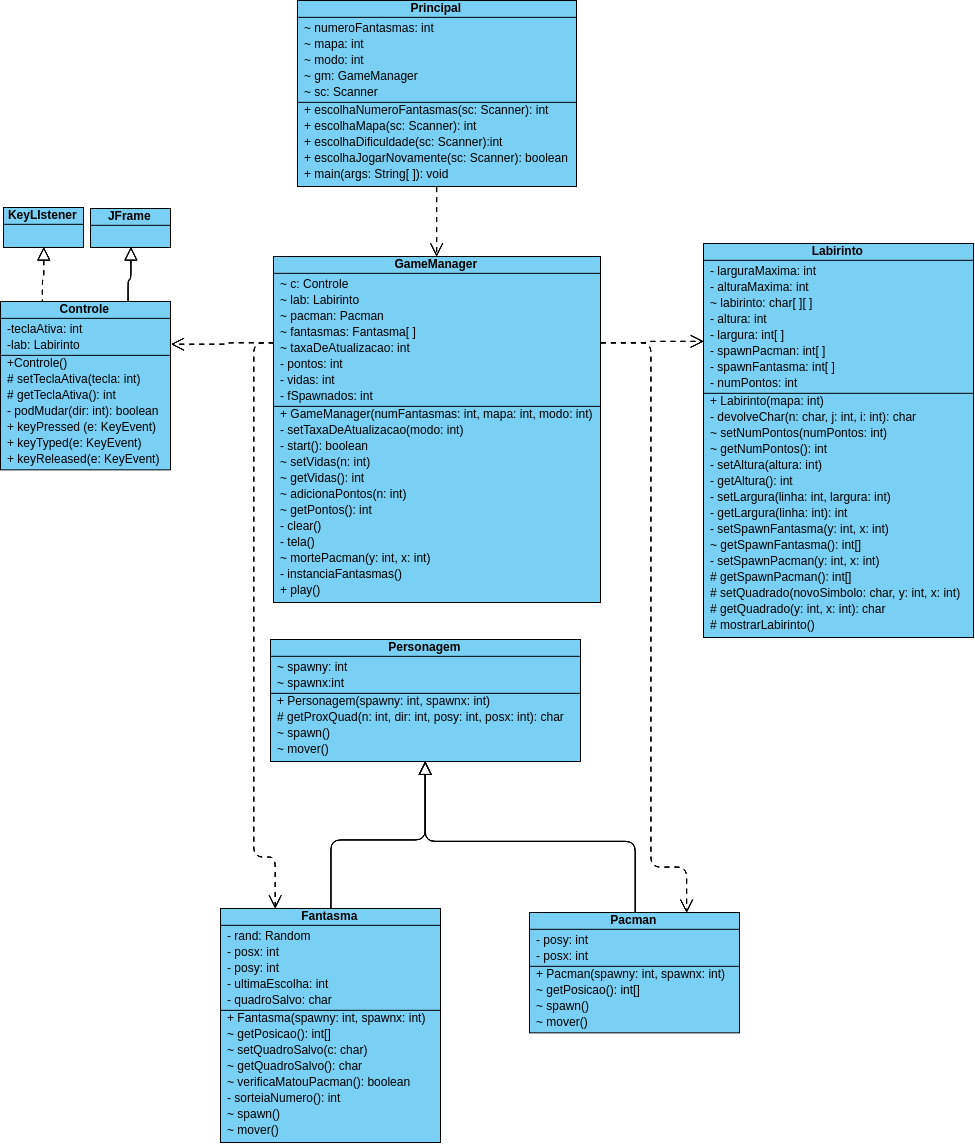
\includegraphics[width=12cm]{UML.png}
\end{center}

\section{Conceitos de orientação a objetos aplicados}
Durante o desenvolvimento do jogo, tentou-se aplicar todos os conceitos de Orientação a Objetos citados na descrição do projeto.

Primeiramente, o \textbf{encapsulamento} foi garantido utilizando o modificador de acesso \textsl{private} para todos os atributos de instância das classes criadas. Essa característica foi endossada pela criação de métodos \textsl{get} e \textsl{set} para tais atributos, a fim de que fossem utilizadas por métodos de todas as classes presentes num pacote comum. No caso de atributos de classe, utilizou-se o modificador default, por considerar-se que tais atributos deveriam ser de acesso a todas as classes neste pacote comum.

Em relação aos métodos de todas as classes, prezou-se pela modulação das funções, de forma a contribuir para uma estrutura geral \textbf{mais coesa}. Neste caso, foi designado o modificador \textsl{private} para métodos que são utilizados apenas pela classe que os possui. Além disso, foram criados métodos para específicas funções, que são utilizados por muitos outros métodos presentes no programa, os quais são baseados na mesma lógica básica. É, por exemplo, o caso do método \texttt{getProxQuad()}, presente na classe abstrata Personagem. Esse método retorna o \textsl{n} próximo quadrado que um personagem (Pac-Man ou fantasma) irá passar, levando em consideração a direção para a qual ele está se direcionando e também sua posição atual. É utilizado por métodos sobrescritos de movimentação presentes em Pacman e Fantasma.

Como já explicitado, utilizou-se o conceito de \textbf{herança} ao criar a classe abstrata Personagem, estendida por Pacman e Fantasma. Neste caso, estas duas outras classas herdam atributos e métodos, sobrescrevendo \texttt{mover()} e \texttt{spawn()}, responsáveis pela movimentação e pelo surgimento do dito personagem, respectivamente.

Também foi implementada a \textbf{sobrecarga de construtor} nas classes GameManager, Labirinto e Personagem, de forma que há necessidade de passar alguns parâmetros para instanciar um novo objeto. No caso de Pacman e Fantasma, o construtor também foi sobrecarregado, devido à necessidade de chamar o construtor da superclasse (Personagem), que, como dito, requer parâmetros.

A \textbf{sobrescrita de métodos} foi utilizada principalmente ao declarar os métodos de movimentação e de surgimento do Pac-Man e dos fantasmas. Isso ocorre pelo fato de que os fantasmas são comandados por aleatoriedade, e o Pac-Man pelo usuário. No entanto, utilizou-se também ao \textbf{implementar} o método \texttt{keyPressed()}, presente na classe Controle. Esse método é sobrescrito da \textbf{interface} KeyListener, e é modificado a fim armazenar, num atributo de classe, as teclas que o usuário pressiona. Tal atributo é utilizado pela classe Pacman, mais precisamente para construir sua movimentação.

Por fim, utilizou-se o \textbf{tratamento de exceções} pontualmente para duas situações. A primeira diz respeito à leitura de um mapa. Se o mapa criado excede o tamanho limite (500x500), definido pelo grupo, então o programa lança uma exceção, alertando tal fato. A segunda se relaciona às exceções que podem ser lançadas pelo método \texttt{sleep()}, importado do pacote \texttt{java.util.concurrent.TimeUnit}, responsável pelo controle de tempo do jogo. Neste caso, o programa alerta que ocorreu um erro, demonstrando sua descrição e encerrando-se em seguida.

Ressalta-se que, durante o desenvolvimento do jogo e ao decorrer das aulas, surgiu a intenção de implementar o padrão de projeto Singleton para formalizar uma instância global de Pacman, Controle, Labirinto e GameManager. No entanto, devido ao limite de tempo e a todo o progresso efetuado antes de tal evento, optou-se por não utilizar o padrão de projeto, mantendo muitos atributos e métodos como \texttt{static}.

\section{Participação de cada integrante do grupo}
Durante a manutenção do projeto, todos os integrantes do grupo discutiram e levantaram ideias de implementação para os recursos, buscando a forma mais eficiente de realizar o desenvolvimento. Além disso, todos os integrantes também ajudaram a resolver eventuais problemas que apareceram no decorrer da construção do jogo. Portanto, por mais que haja determinada separação de responsabilidades nesta seção, na maioria dos casos as funcionalidades foram desenvolvidas em conjunto, sendo aprimoradas ao longo do tempo de trabalho.

\textbf{André Aranovich Florentino}: Implementação da leitura e criação do labirinto a partir de um arquivo de texto, revisão de código, montagem do diagrama de classes no formato UML.

\textbf{Bruno Tatsuya Masunaga Santos}: Implementação da estrutura de captura de teclas pressionadas pelo usuário, desenvolvimento do movimento dos personagens, otimização de casos do fluxo de jogo (como morte do Pac-Man e game-over), habilitação de parâmetros de entrada para o programa (número de fantasmas, mapa, dificuldade), elaboração parcial do relatório.

\textbf{Lucas Eduardo Gonçalves da Rosa}:

\textbf{Wesley Pereira da Silva}:

\end{document}